\documentclass{standalone}
\usepackage{graphicx}	
\usepackage{amssymb, amsmath}
\usepackage{color}

\usepackage{tikz}
\usetikzlibrary{calc, arrows.meta}
\usepackage{pgfmath}

\definecolor{light}{RGB}{220, 188, 188}
\definecolor{mid}{RGB}{185, 124, 124}
\definecolor{dark}{RGB}{143, 39, 39}
\definecolor{highlight}{RGB}{180, 31, 180}
\definecolor{gray10}{gray}{0.1}
\definecolor{gray20}{gray}{0.2}
\definecolor{gray30}{gray}{0.3}
\definecolor{gray40}{gray}{0.4}
\definecolor{gray60}{gray}{0.6}
\definecolor{gray70}{gray}{0.7}
\definecolor{gray80}{gray}{0.8}
\definecolor{gray90}{gray}{0.9}
\definecolor{gray95}{gray}{0.95}

\newcommand*{\offset}{0.025}

\begin{document}

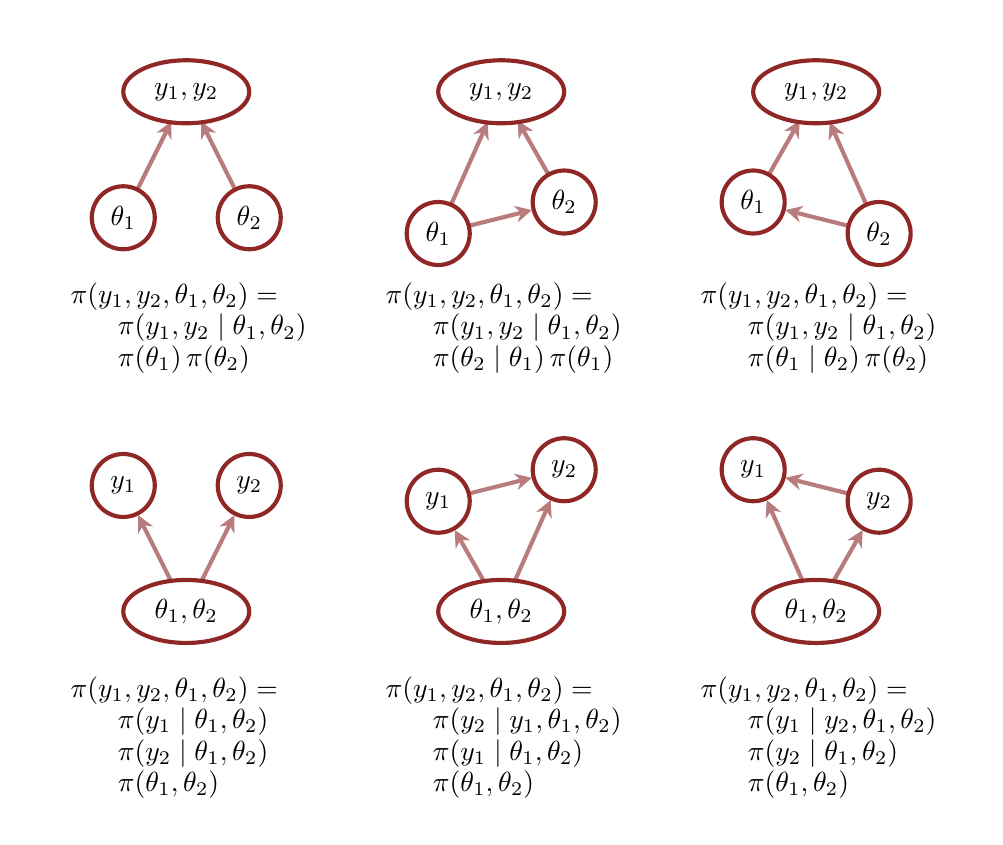
\begin{tikzpicture}[scale=0.2, thick]

  \begin{scope}[shift={(0, 0)}]
    \draw[white] (-10, -17) rectangle (10, 8);
  
    \pgfmathsetmacro{\r}{2}
  
    \coordinate (A) at (-4, -4);
    \coordinate (B) at (+4, -4);
    \coordinate (C) at (0, +4);
  
    \draw[-{Stealth[length=6pt, width=6pt]}, shorten >=12, color=mid, line width=1.5] (A) -- (C);
    \draw[-{Stealth[length=6pt, width=6pt]}, shorten >=12, color=mid, line width=1.5] (B) -- (C);
    
    \node[anchor=west] at (-8, -9) { $\pi(y_{1}, y_{2}, \theta_{1}, \theta_{2}) = $ };
    \node[anchor=west] at (-5, -11) { $\pi(y_{1}, y_{2} \mid \theta_{1}, \theta_{2})$ };
    \node[anchor=west] at (-5, -13) { $\pi(\theta_{1}) \, \pi(\theta_{2})$ };
  
    \filldraw[fill=white, draw=dark, line width=1.5] (A) circle (\r)
    node[color=black] { $\theta_{1}$ };

    \filldraw[fill=white, draw=dark, line width=1.5] (B) circle (\r)
    node[color=black] { $\theta_{2}$ };
      
    \filldraw[fill=white, draw=dark, line width=1.5] (C) circle [x radius={2 * \r}, y radius={\r}]
    node[color=black] { $y_{1}, y_{2}$ };
  \end{scope}

  \begin{scope}[shift={(20, 0)}]
    \draw[white] (-10, -17) rectangle (10, 8);
  
    \pgfmathsetmacro{\r}{2}
  
    \coordinate (A) at (-4, -5);
    \coordinate (B) at (+4, -3);
    \coordinate (C) at (0, +4);
  
    \draw[-{Stealth[length=6pt, width=6pt]}, shorten >=12, color=mid, line width=1.5] (A) -- (C);
    \draw[-{Stealth[length=6pt, width=6pt]}, shorten >=12, color=mid, line width=1.5] (A) -- (B);
    \draw[-{Stealth[length=6pt, width=6pt]}, shorten >=12, color=mid, line width=1.5] (B) -- (C);
    
    \node[anchor=west] at (-8, -9) { $\pi(y_{1}, y_{2}, \theta_{1}, \theta_{2}) = $ };
    \node[anchor=west] at (-5, -11) { $\pi(y_{1}, y_{2} \mid \theta_{1}, \theta_{2})$ };
    \node[anchor=west] at (-5, -13) { $\pi(\theta_{2} \mid \theta_{1}) \, \pi(\theta_{1})$ };
  
    \filldraw[fill=white, draw=dark, line width=1.5] (A) circle (\r)
    node[color=black] { $\theta_{1}$ };

    \filldraw[fill=white, draw=dark, line width=1.5] (B) circle (\r)
    node[color=black] { $\theta_{2}$ };
      
    \filldraw[fill=white, draw=dark, line width=1.5] (C) circle [x radius={2 * \r}, y radius={\r}]
    node[color=black] { $y_{1}, y_{2}$ };
  \end{scope}

  \begin{scope}[shift={(40, 0)}]
    \draw[white] (-10, -17) rectangle (10, 8);
  
    \pgfmathsetmacro{\r}{2}
  
    \coordinate (A) at (-4, -3);
    \coordinate (B) at (+4, -5);
    \coordinate (C) at (0, +4);
  
    \draw[-{Stealth[length=6pt, width=6pt]}, shorten >=12, color=mid, line width=1.5] (A) -- (C);
    \draw[-{Stealth[length=6pt, width=6pt]}, shorten >=12, color=mid, line width=1.5] (B) -- (C);
    \draw[-{Stealth[length=6pt, width=6pt]}, shorten >=12, color=mid, line width=1.5] (B) -- (A);
    
    \node[anchor=west] at (-8, -9) { $\pi(y_{1}, y_{2}, \theta_{1}, \theta_{2}) = $ };
    \node[anchor=west] at (-5, -11) { $\pi(y_{1}, y_{2} \mid \theta_{1}, \theta_{2})$ };
    \node[anchor=west] at (-5, -13) { $\pi(\theta_{1} \mid \theta_{2}) \, \pi(\theta_{2})$ };
  
    \filldraw[fill=white, draw=dark, line width=1.5] (A) circle (\r)
    node[color=black] { $\theta_{1}$ };

    \filldraw[fill=white, draw=dark, line width=1.5] (B) circle (\r)
    node[color=black] { $\theta_{2}$ };
      
    \filldraw[fill=white, draw=dark, line width=1.5] (C) circle [x radius={2 * \r}, y radius={\r}]
    node[color=black] { $y_{1}, y_{2}$ };
  \end{scope}


  \begin{scope}[shift={(0, -25)}]
    \draw[white] (-10, -17) rectangle (10, 8);
  
    \pgfmathsetmacro{\r}{2}
  
    \coordinate (A) at (0, -4);
    \coordinate (B) at (-4, +4);
    \coordinate (C) at (+4, +4);
  
    \draw[-{Stealth[length=6pt, width=6pt]}, shorten >=12, color=mid, line width=1.5] (A) -- (B);
    \draw[-{Stealth[length=6pt, width=6pt]}, shorten >=12, color=mid, line width=1.5] (A) -- (C);
    
    \node[anchor=west] at (-8, -9) { $\pi(y_{1}, y_{2}, \theta_{1}, \theta_{2}) = $ };
    \node[anchor=west] at (-5, -11) { $\pi(y_{1} \mid \theta_{1}, \theta_{2})$ };
    \node[anchor=west] at (-5, -13) { $\pi(y_{2} \mid \theta_{1}, \theta_{2})$ };
    \node[anchor=west] at (-5, -15) { $\pi(\theta_{1}, \theta_{2})$ };
  
    \filldraw[fill=white, draw=dark, line width=1.5] (A) circle [x radius={2 * \r}, y radius={\r}]
    node[color=black] { $\theta_{1}, \theta_{2}$ };
      
    \filldraw[fill=white, draw=dark, line width=1.5] (B) circle (\r)
    node[color=black] { $y_{1}$ };
    
    \filldraw[fill=white, draw=dark, line width=1.5] (C) circle (\r)
    node[color=black] { $y_{2}$ };
  \end{scope}

  \begin{scope}[shift={(20, -25)}]
    \draw[white] (-10, -17) rectangle (10, 8);
  
    \pgfmathsetmacro{\r}{2}
  
    \coordinate (A) at (0, -4);
    \coordinate (B) at (-4, +3);
    \coordinate (C) at (+4, +5);
  
    \draw[-{Stealth[length=6pt, width=6pt]}, shorten >=12, color=mid, line width=1.5] (A) -- (B);
    \draw[-{Stealth[length=6pt, width=6pt]}, shorten >=12, color=mid, line width=1.5] (B) -- (C);
    \draw[-{Stealth[length=6pt, width=6pt]}, shorten >=12, color=mid, line width=1.5] (A) -- (C);
    
    \node[anchor=west] at (-8, -9) { $\pi(y_{1}, y_{2}, \theta_{1}, \theta_{2}) = $ };
    \node[anchor=west] at (-5, -11) { $\pi(y_{2} \mid y_{1}, \theta_{1}, \theta_{2})$ };
    \node[anchor=west] at (-5, -13) { $\pi(y_{1} \mid \theta_{1}, \theta_{2})$ };
    \node[anchor=west] at (-5, -15) { $\pi(\theta_{1}, \theta_{2})$ };
  
    \filldraw[fill=white, draw=dark, line width=1.5] (A) circle [x radius={2 * \r}, y radius={\r}]
    node[color=black] { $\theta_{1}, \theta_{2}$ };
      
    \filldraw[fill=white, draw=dark, line width=1.5] (B) circle (\r)
    node[color=black] { $y_{1}$ };
    
    \filldraw[fill=white, draw=dark, line width=1.5] (C) circle (\r)
    node[color=black] { $y_{2}$ };
  \end{scope}
  
  \begin{scope}[shift={(40, -25)}]
    \draw[white] (-10, -17) rectangle (10, 8);
  
    \pgfmathsetmacro{\r}{2}
  
    \coordinate (A) at (0, -4);
    \coordinate (B) at (-4, +5);
    \coordinate (C) at (+4, +3);
  
    \draw[-{Stealth[length=6pt, width=6pt]}, shorten >=12, color=mid, line width=1.5] (A) -- (B);
    \draw[-{Stealth[length=6pt, width=6pt]}, shorten >=12, color=mid, line width=1.5] (A) -- (C);
    \draw[-{Stealth[length=6pt, width=6pt]}, shorten >=12, color=mid, line width=1.5] (C) -- (B);
    
    \node[anchor=west] at (-8, -9) { $\pi(y_{1}, y_{2}, \theta_{1}, \theta_{2}) = $ };
    \node[anchor=west] at (-5, -11) { $\pi(y_{1} \mid y_{2}, \theta_{1}, \theta_{2})$ };
    \node[anchor=west] at (-5, -13) { $\pi(y_{2} \mid \theta_{1}, \theta_{2})$ };
    \node[anchor=west] at (-5, -15) { $\pi(\theta_{1}, \theta_{2})$ };
  
    \filldraw[fill=white, draw=dark, line width=1.5] (A) circle [x radius={2 * \r}, y radius={\r}]
    node[color=black] { $\theta_{1}, \theta_{2}$ };
      
    \filldraw[fill=white, draw=dark, line width=1.5] (B) circle (\r)
    node[color=black] { $y_{1}$ };
    
    \filldraw[fill=white, draw=dark, line width=1.5] (C) circle (\r)
    node[color=black] { $y_{2}$ };
  \end{scope}

\end{tikzpicture}

\end{document}  